\documentclass[journal,12pt,twocolumn]{IEEEtran}

\usepackage{setspace}
\usepackage{gensymb}
\singlespacing
\usepackage[cmex10]{amsmath}

\usepackage{amsthm}

\usepackage{mathrsfs}
\usepackage{txfonts}
\usepackage{stfloats}
\usepackage{bm}
\usepackage{cite}
\usepackage{cases}
\usepackage{subfig}

\usepackage{longtable}
\usepackage{multirow}

\usepackage{enumitem}
\usepackage{mathtools}
\usepackage{steinmetz}
\usepackage{tikz}
\usepackage{circuitikz}
\usepackage{verbatim}
\usepackage{tfrupee}
\usepackage[breaklinks=true]{hyperref}
\usepackage{graphicx}
\usepackage{tkz-euclide}

\usetikzlibrary{calc,math}
\usepackage{listings}
    \usepackage{color}                                            %%
    \usepackage{array}                                            %%
    \usepackage{longtable}                                        %%
    \usepackage{calc}                                             %%
    \usepackage{multirow}                                         %%
    \usepackage{hhline}                                           %%
    \usepackage{ifthen}                                           %%
    \usepackage{lscape}     
\usepackage{multicol}
\usepackage{chngcntr}

\DeclareMathOperator*{\Res}{Res}

\renewcommand\thesection{\arabic{section}}
\renewcommand\thesubsection{\thesection.\arabic{subsection}}
\renewcommand\thesubsubsection{\thesubsection.\arabic{subsubsection}}

\renewcommand\thesectiondis{\arabic{section}}
\renewcommand\thesubsectiondis{\thesectiondis.\arabic{subsection}}
\renewcommand\thesubsubsectiondis{\thesubsectiondis.\arabic{subsubsection}}


\hyphenation{op-tical net-works semi-conduc-tor}
\def\inputGnumericTable{}                                 %%

\lstset{
%language=C,
frame=single, 
breaklines=true,
columns=fullflexible
}
\begin{document}

\newcommand{\BEQA}{\begin{eqnarray}}
\newcommand{\EEQA}{\end{eqnarray}}
\newcommand{\define}{\stackrel{\triangle}{=}}
\bibliographystyle{IEEEtran}
\raggedbottom
\setlength{\parindent}{0pt}
\providecommand{\mbf}{\mathbf}
\providecommand{\pr}[1]{\ensuremath{\Pr\left(#1\right)}}
\providecommand{\qfunc}[1]{\ensuremath{Q\left(#1\right)}}
\providecommand{\sbrak}[1]{\ensuremath{{}\left[#1\right]}}
\providecommand{\lsbrak}[1]{\ensuremath{{}\left[#1\right.}}
\providecommand{\rsbrak}[1]{\ensuremath{{}\left.#1\right]}}
\providecommand{\brak}[1]{\ensuremath{\left(#1\right)}}
\providecommand{\lbrak}[1]{\ensuremath{\left(#1\right.}}
\providecommand{\rbrak}[1]{\ensuremath{\left.#1\right)}}
\providecommand{\cbrak}[1]{\ensuremath{\left\{#1\right\}}}
\providecommand{\lcbrak}[1]{\ensuremath{\left\{#1\right.}}
\providecommand{\rcbrak}[1]{\ensuremath{\left.#1\right\}}}
\theoremstyle{remark}
\newtheorem{rem}{Remark}
\newcommand{\sgn}{\mathop{\mathrm{sgn}}}
\providecommand{\abs}[1]{\vert#1\vert}
\providecommand{\res}[1]{\Res\displaylimits_{#1}} 
\providecommand{\norm}[1]{\lVert#1\rVert}
%\providecommand{\norm}[1]{\lVert#1\rVert}
\providecommand{\mtx}[1]{\mathbf{#1}}
\providecommand{\mean}[1]{E[ #1 ]}
\providecommand{\fourier}{\overset{\mathcal{F}}{ \rightleftharpoons}}
%\providecommand{\hilbert}{\overset{\mathcal{H}}{ \rightleftharpoons}}
\providecommand{\system}{\overset{\mathcal{H}}{ \longleftrightarrow}}
	%\newcommand{\solution}[2]{\textbf{Solution:}{#1}}
\newcommand{\solution}{\noindent \textbf{Solution: }}
\newcommand{\cosec}{\,\text{cosec}\,}
\providecommand{\dec}[2]{\ensuremath{\overset{#1}{\underset{#2}{\gtrless}}}}
\newcommand{\myvec}[1]{\ensuremath{\begin{pmatrix}#1\end{pmatrix}}}
\newcommand{\mydet}[1]{\ensuremath{\begin{vmatrix}#1\end{vmatrix}}}
\numberwithin{equation}{subsection}
\makeatletter
\@addtoreset{figure}{problem}
\makeatother
\let\StandardTheFigure\thefigure
\let\vec\mathbf
\renewcommand{\thefigure}{\theproblem}
\def\putbox#1#2#3{\makebox[0in][l]{\makebox[#1][l]{}\raisebox{\baselineskip}[0in][0in]{\raisebox{#2}[0in][0in]{#3}}}}
     \def\rightbox#1{\makebox[0in][r]{#1}}
     \def\centbox#1{\makebox[0in]{#1}}
     \def\topbox#1{\raisebox{-\baselineskip}[0in][0in]{#1}}
     \def\midbox#1{\raisebox{-0.5\baselineskip}[0in][0in]{#1}}
\vspace{3cm}
\title{Assignment 4}%number
\author{Amulya Tallamraju - AI20BTECH11003}
\maketitle
\newpage
\bigskip
\renewcommand{\thefigure}{\theenumi}
\renewcommand{\thetable}{\theenumi}
\newcommand*{\permcomb}[4][0mu]{{{}^{#3}\mkern#1#2_{#4}}}
\newcommand*{\perm}[1][-3mu]{\permcomb[#1]{P}}
\newcommand*{\comb}[1][-1mu]{\permcomb[#1]{C}}
Download all python codes from 
\begin{lstlisting}
https://github.com/AmulyaTallamraju/Assignment-4/blob/main/Assignment4/codes/Assignment-4.py
\end{lstlisting}
%
and latex-tikz codes from 
%
\begin{lstlisting}
https://github.com/AmulyaTallamraju/Assignment-4/blob/main/Assignment4/Assignment-4.tex
\end{lstlisting}
\section*{GATE 2018 MA - Q.54}
Let $X_1$ and $X_2$ be independent geometric random variables with the same probability
mass function given by $\pr{X = k} = p(1-p)^{k-1}$
, $k = 1, 2, \ldots$ Then the value of
$\pr{X_1 = 2 | X_1 + X_2 = 4}$ correct up to three decimal places is
\section*{Solution}
Let 
\begin{align}
\label{eq:dice_pmf_xi}
p_{X_i}(k)=\pr{X_i=k}=
\begin{cases}
p(1-p)^{k-1} & n=1,2,...
\\
0 & otherwise
\end{cases}
\end{align}
where i=1,2
\begin{align}
\pr{A|B}=\frac{\pr{AB}}{\pr{B}}
\end{align}
\begin{align}
(X_1 = 2) \cap (X_1 + X_2 = 4)=\brak{X_1=2,X_2=2}
\end{align}
Thus,
\begin{align}
  \pr{X_1 = 2 | X_1 + X_2 = 4}&=\frac{\pr{X_1=2,X_2=2}}{\pr{X_1+X_2=4}}
 \end{align}
 Since the two events are independent,
\begin{align}\label{result}
  \pr{X_1 = 2 | X_1 + X_2 = 4}=\frac{\pr{X_1=2}\pr{X_2=2}}{\pr{X_1+X_2=4}}
 \end{align}
Let
\begin{align}\label{eq:dice_xdef}
X=X_1+X_2
\end{align}
From \eqref{eq:dice_xdef},
\begin{align}
p_X(n) &= \pr{X_1 + X_2 = n} = \pr{X_1  = n -X_2}
\\
&= \sum_{k}^{}\pr{X_1  = n -k | X_2 = k}p_{X_2}(k)
\label{eq:dice_x_sum}
\end{align}
after unconditioning.  $\because X_1$ and $X_2$ are independent,
\begin{multline}
\pr{X_1  = n -k | X_2 = k} 
\\
= \pr{X_1  = n -k}
= p_{X_1}(n-k)
\label{eq:dice_x1_indep}
\end{multline}
From \eqref{eq:dice_x_sum} and \eqref{eq:dice_x1_indep},
\begin{align}
p_X(n) = \sum_{k}^{}p_{X_1}(n-k)p_{X_2}(k) = p_{X_1}(n)*p_{X_2}(n)
\label{eq:dice_x_conv}
\end{align}
where $*$ denotes the convolution operation. 
%\cite{proakis_dsp}.  
Substituting from \eqref{eq:dice_pmf_xi}
in \eqref{eq:dice_x_conv},
\begin{align}
p_X(n)& = \sum_{k=1}^{n-1}p_{X_1}(n-k)p_{X_2}(k)\\
& = \sum_{k=1}^{n-1} (1-p)^{k-1} p \cdot (1-p)^{n-k-1} p \\ & = (1-p)^{n-2} p^2 \sum_{k=1}^{n-1} 1 \\& = (n-1) (1-p)^{n-2}p^2\label{ref}\end{align}
From \eqref{ref} and \eqref{eq:dice_pmf_xi} we have
\begin{align}
&\pr{X_1=2}=\pr{X_2=2}=p(1-p)\\
&\pr{X_1+X_2=4}=3(1-p)^2p^2
\end{align}
Substituting in \eqref{result}
\begin{align}
 \pr{X_1 = 2 | X_1 + X_2 = 4}
 &=\frac{(1-p)^2p^2}{3(1-p)^2p^2}\\
 &=\frac{1}{3}
\end{align}
Therefore, the value of
$\pr{X_1 = 2 | X_1 + X_2 = 4}$ correct up to three decimal places is 0.333
\begin{figure}[h]
    \centering
    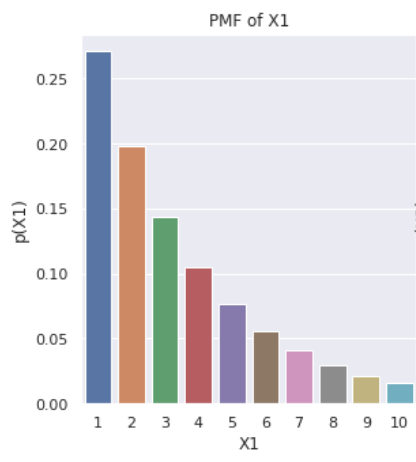
\includegraphics[width=\columnwidth]{1.png}
    \caption{PMF of $X_1$ when p=0.27047335  }
    \label{1}
\end{figure}[h]
\begin{figure}
    \centering
    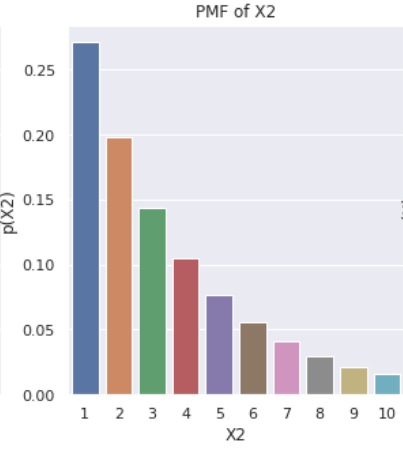
\includegraphics[width=\columnwidth]{2.png}
    \caption{PMF of $X_2$ when p=0.27047335  }
    \label{2}
\end{figure}
\begin{figure}[h!]
    \centering
    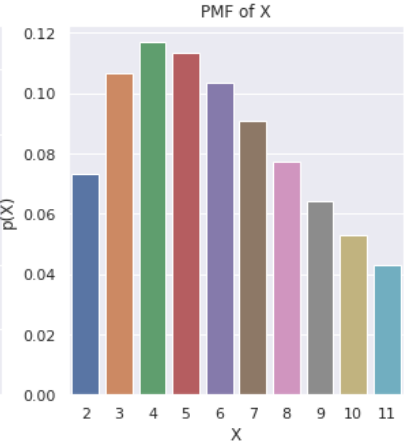
\includegraphics[width=\columnwidth]{3.png}
    \caption{PMF of $X$ when p=0.27047335  }
    \label{3}
\end{figure}
\end{document}
